\documentclass[12pt,spanish,fleqn,openany,letterpaper,pagesize]{scrbook}

\usepackage[utf8]{inputenc}
\usepackage[spanish]{babel}
\usepackage{fancyhdr}
\usepackage{epsfig}
\usepackage{epic}
\usepackage{eepic}
\usepackage{amsmath}
\usepackage{threeparttable}
\usepackage{amscd}
\usepackage{here}
\usepackage{graphicx}
\usepackage{lscape}
\usepackage{tabularx}
\usepackage{subfigure}
\usepackage{longtable}


\usepackage{rotating} %Para rotar texto, objetos y tablas seite. No se ve en DVI solo en PS. Seite 328 Hundebuch
                        %se usa junto con \rotate, \sidewidestable ....


\renewcommand{\theequation}{\thechapter-\arabic{equation}}
\renewcommand{\thefigure}{\textbf{\thechapter-\arabic{figure}}}
\renewcommand{\thetable}{\textbf{\thechapter-\arabic{table}}}


\pagestyle{fancyplain}%\addtolength{\headwidth}{\marginparwidth}
\textheight22.5cm \topmargin0cm \textwidth16.5cm
\oddsidemargin0.5cm \evensidemargin-0.5cm%
\renewcommand{\chaptermark}[1]{\markboth{\thechapter\; #1}{}}
\renewcommand{\sectionmark}[1]{\markright{\thesection\; #1}}
\lhead[\fancyplain{}{\thepage}]{\fancyplain{}{\rightmark}}
\rhead[\fancyplain{}{\leftmark}]{\fancyplain{}{\thepage}}
\fancyfoot{}
\thispagestyle{fancy}%


\addtolength{\headwidth}{0cm}
\unitlength1mm %Define la unidad LE para Figuras
\mathindent0cm %Define la distancia de las formulas al texto,  fleqn las descentra
\marginparwidth0cm
\parindent0cm %Define la distancia de la primera linea de un parrafo a la margen

%Para tablas,  redefine el backschlash en tablas donde se define la posici\'{o}n del texto en las
%casillas (con \centering \raggedright o \raggedleft)
\newcommand{\PreserveBackslash}[1]{\let\temp=\\#1\let\\=\temp}
\let\PBS=\PreserveBackslash

%Espacio entre lineas
\renewcommand{\baselinestretch}{1.1}

%Neuer Befehl f\"{u}r die Tabelle Eigenschaften der Aktivkohlen
\newcommand{\arr}[1]{\raisebox{1.5ex}[0cm][0cm]{#1}}

%Neue Kommandos
\usepackage{Befehle}


%Trennungsliste
\hyphenation {Reaktor-ab-me-ssun-gen Gas-zu-sa-mmen-set-zung
Raum-gesch-win-dig-keit Durch-fluss Stick-stoff-gemisch
Ad-sorp-tions-tem-pe-ra-tur Klein-schmidt
Kohlen-stoff-Mole-kular-siebe Py-rolysat-aus-beu-te
Trans-port-vor-gan-ge}


\begin{document}

\chapter{Marco Teorico}

\section{Epidemiología Panorámica}

\justifying


\par La \textit{Teledetección} se define como el proceso de adquirir
  información acerca de un objeto, área o fenómeno desde la distancia.
  Un sensor remoto es un instrumento capaz de realizar percepción remota, por lo
  que en esta amplia definición caben desde los ojos hasta los
  radiotelescopios.

\par Existen dos grandes tipos de sensores remotos (SR): activos y pasivos.
  Los activos son aquellos que obtienen la información generando su propia energía
  mientras que los pasivos dependen de una fuente externa, que en la Tierra
  principalmente proviene del Sol. Hasta el día de hoy, los más usados son los
  sensores pasivos dado que permiten medir la magnitud de la radiación electromagnética
  reflejada e irradiada desde la superficie de la Tierra y de la atmósfera y,
  de esta manera, derivar información sobre las condiciones de la superficie \cite{cami_tartagal}.


\par Los SR más utilizados y con mayor cantidad de aplicaciones son los que se
  encuentran a bordo de satélites que orbitan sobre la Tierra, bien sea
  en órbitas geoestacionarias\footnote{Están en altitudes entre 23000 y 40000 km,
  sobre la franja ecuatorial y viaja a la misma velocidad de rotación de la Tierra
  por lo que siempre están fijos sobre un punto determinado de la superficie terrestre},
  u órbitas polares, aquellas que pasan repetidamente por diferentes áreas
  de la Tierra mientras están orbitando alrededor del planeta a altitudes menores.


\par Las tecnologías relacionadas al ámbito aeroespacial dieron lugar a programas
  que integran estas tecnologías con,
  por ejemplo, la agricultura, salud pública, geología y las ciencias forestales.
  A su vez, la información obtenida por dichos SR se puede aplicar a estudios
  entomológicos\footnote{De insectos}, debido a que ellos proveen gran cantidad
  y diversidad de información sobre la cobertura de la Tierra: características
  de la vegetación, cuerpos de agua, temperaturas, entre otras. Ésta, también es
  información sobre el hábitat de insectos y artrópodos vectores \cite{estallo_ndwi, data_driven_prediction},
  y, por lo tanto, de acuerdo a la teoría de Pavlovsky \cite{nidality} en la que
  expone la correlación entre el hábitat y enfermedades transmitidas por vectores,
  los datos de los SR se pueden utilizar como fuente de información sobre la
  distribución espacio-temporal de dichas afecciones.


\par Con la acumulación de datos registrados por sensores remotos desde los años
  70 existen series temporales que permiten realizar varios tipos de análisis con
  relevancia para la transmisión de la enfermedad de Dengue y otras
  ETV\footnote{Enfermedades de Transmisión Vectorial}.
  Entre ellas, series temporales de imágenes de mediana resolución espacial
  permiten analizar en perspectiva histórica los cambios de uso y cobertura del
  terreno, proceso que habitualmente tiene vinculación con cambios en la
  epidemiología de la enfermedad \cite{german_temporal}.
  A su vez, el deterioro de las condiciones de salud en el mundo, el avance significativo
  en el procesamiento de computadoras, la mejora en la adquisición de datos,
  la reducción de los costos de hardware y software y el desarrollo de tecnología
  GIS\footnote{Sistema de Información Geográfica} han llevado al lanzamiento
  de programas que apuntan a integrar SR / GIS en aplicaciones de salud
  \cite{tesis_riesgo_viral, tesis_gonza, espinosa_temporal, rs_public_health}.



\par El uso de técnicas de Teledetección para mapear la distribución de vectores y el riesgo
  de enfermedades ha tenido una gran evolución durante las últimas dos
  décadas (13). La complejidad de las técnicas va desde el uso de simples
  correlaciones entre las firmas espectrales de diferentes coberturas, usos del
  suelo y abundancia de especies (26,27) hasta técnicas complejas que integran variables
  ambientales obtenidas de satélites con la biología de los vectores (13).
  Estas técnicas se usan para desarrollar modelos predictivos de riesgo,
  los cuales principalmente se realizan a través de técnicas estadísticas de
  regresión logística y análisis discriminante, que dilucidan las asociaciones
  entre datos ambientales multivariados y los patrones de presencia o ausencia de
  vectores para así mapear los vectores o las enfermedades.
  Estos métodos son capaces de predecir la probabilidad “\textit{a posteriori}” de la
  presencia de la variable dependiente (vector o enfermedad), a partir de un
  grupo de variables independientes (datos de clima y cobertura de la tierra) y de esta
  forma pueden ser usados para hacer mapas de riesgo a partir de bases de datos.


  \begin{figure}
  \centering%
  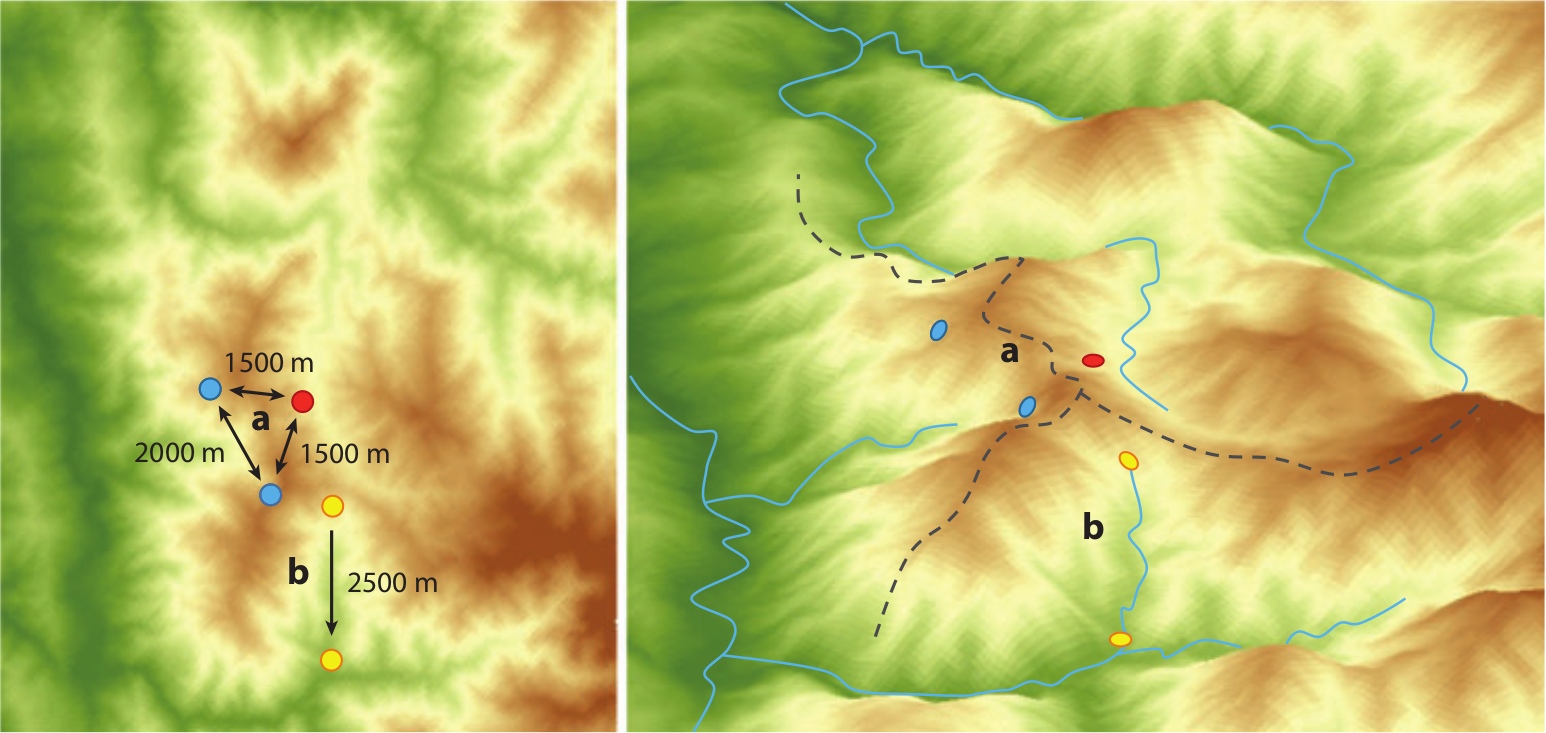
\includegraphics[width=1\textwidth]{images/paisajes_heterogeneos}%
  \caption{La propagación y persistencia a través de paisajes heterogéneos}\label{fig:paisajes_h}
  \end{figure}

% la vision panotamira de los problemas de este tipo esta vinculada con la
% el hecho de que dichos problemas dependen de un entorno no local
\par Las condiciones ambientales que determinan la
  conectividad \footnote{El grado en que el paisaje impide o facilita el movimiento
  entre las zonas de recursos \cite{landscape_connectivity}} de los paisajes
  para la disperción pueden variar en las distintas regiones y dependen de cómo
  el patógeno se dispersa biológicamente (e.j: dado un patógeno portado por
  vectores, el movimiento del insecto) o abióticamente (e.j: flujos de viento o agua).
  Por ejemplo, rios y corrientes pueden actuar como corredores de disperción que
  fomentan la propagación de la infección a través de paisajes heterogéneos
  para patógenos de plantas transmitidos por el agua (53), mientras que en otros
  sistemas, como las enfermedades zoonóticas de mamíferos terrestres, estos mismos
  cuerpos de agua pueden funcionar como barreras impidiendo el movimiento
  del huesped o del vector (97). Éstas condiciones se ven reflejadas en la
  Figura \ref{fig:paisajes_h} de \cite{Landscape Epidemiology of Emerging Infectious...}.
  Notemos que en el caso de \textbf{a)}, la
  conectividad entre los sitios azules es mayor que la que se da entre éstos y
  los amarillos, y también entre ellos y los rojos, siendo que la distancia
  Euclidea entre los azules es mayor. Ésto ocurre porque el sitio rojo está del otro lado
  de la cordillera, la cual funciona como una barrera geográfica para la
  inoculación\footnote{Introducción de microorganismos vivos, muertos o atenuados,
  en un organismo de forma accidental o voluntaria.}, el huésped y/o la disperción
  del vector. En el caso \textbf{b)}, en cambio, se da la situación de un
  patosistema\footnote{Subsistema dentro del sistema agrícola caracterizado por el
  fenómeno de parasitismo. Está constituido por un hospedante susceptible,
  un patógeno virulento y un ambiente predispuesto a la enfermedad} acuático, en
  donde la inoculación sucede a través del agua: los dos sitios amarillos son los
  más estrechamente conectados, a pesar de que están separados por una mayor
  distancia Euclidea que con otros, porque el sitio amarillo de abajo está localizado
  bajo una corriente que va desde el sitio amarillo de arriba.
% con un así se pega acá
  \par La \textbf{\textit{Epidemiología Panorámica}}\cite{nidality, ostfeld_re_emerging}
  (EP) está estrechamente relacionada a su paralela ecológica, la Ecología
  Panorámica, una ciencia con inicios en los años 1930s que se dedica a estudiar
  las interacciones entre los ambientes y la vegetación (122).
  Sin embargo, los paisajes son espacial y temporalmente dinámicos.
  En simultáneo con el nacimiento de la ecología panorámica como una ciencia,
  Pavlosky estipula el concepto de \textit{nidalidad}\footnote{Se define como
  el foco de la infección. Además, Pavlosky, establece que los focos de
  enfermedades a microescala están determinados por todo el ecosistema \cite{nidality}}
  (o focalidad) de las enfermedades, donde los patógenos son asociados
  a paisajes (zonas) específicos. Un foco de infección contiene tres elementos
  críticos \cite{reisen_landscape}:
  \begin{enumerate}
    \item Vectores con capacidad de transmisión de la infección
    \item Vertebrados capaces de funcionar como reservorio de la infección
    \item Huéspedes susceptibles, como humanos o animales domésticos
  \end{enumerate}
  El concepto de \textit{focalidad} mezclado con la ecología panorámica
  llevó al nacimiento de la ciencia contemporánea
  \textbf{\textit{Epidemiología Panorámica}}, en la cual las enfermedades
  pueden ser asociadas a distintas características del paisaje o cómo
  la configuración entre el vector, el huésped y el patógeno se intersecan
  dado un clima permisivo para que ello suceda.

\par Por definición, la \textit{EP} integra conceptos y
  enfoques de la ecología vinculada a las enfermedades, con el análisis a
  macroescala de la ecología del paisaje. La intersección de estas perspectivas
  nos habilita a entender cómo es que la configuración espacial y las
  características de la composición del paisaje afectan a los procesos
  epidemiológicos a lo largo y ancho de las áreas geográficas que se
  extienden más allá de los procesos que operan localmente dentro de una sola comunidad.
  Así, la \textit{EP} es más que simplemente establecer
  sectores en el territorio y examinar diferencias en condiciones locales de
  factores bióticos y abióticos entre distintos lugares; la clave es obtener
  información sobre la distribución geográfica de la enfermedad y comprender
  cómo las interrelaciones de los paisajes influencian las intereacciones entre
  individuos susceptibles e infectados.

\par La EP ha sido aplicada en gran variedad de estudios sobre vectores de
  enfermedades (28-37). A nivel global, se pueden encontrar contribuciones en esta área
  [32, 33, 34] también con algunas experiencias de herramientas operativas [35].
  A su vez, muchos estudios interdisciplinarios fueron llevados a cabo en
  latinoamérica enfocados en la generación de modelos predictivos de riesgo,
  espaciales y temporales, basados en condiciones ambientales derivadas de
  información satelital [24, 25, 26, 27].
  Por ejemplo, en México, Dumonteil y Gourbiere (38)
  estudiaron la relación entre la distribución de la especie Triatoma dimidiata
  y factores bioclimáticos, para de esta forma desarrollar un modelo predictivo de
  la abundancia domiciliaria por esta especie y las tasas de infección
  por T. cruzi. Estas predicciones se usaron para construir el primer mapa de
  riesgo de transmisión en la península de Yucatán hallándose que la abundancia de T.
  dimidiata se asocia de forma positiva (por análisis de regresión de Poisson)
  con los cultivos, pastos, precipitación, humedad relativa y la temperatura
  máxima. En particular, en Argentina existen varias experiencias en esta
  dirección, [28, 29, 30] abordan el problema de la epidemia del Dengue dando
  herramientas operacionales [31].

\par Por ejemplo, en 2011, Argentina comenzó a desarrollar un proyecto operacional
  (Sistema de Alerta Temprana de Salud, HEWS), útil tanto para las autoridades de
  salud como para los investigadores.
  Básicamente, HEWS es un mapeo de riesgo dinámico del dengue para todas las
  ciudades del país. En este producto, cada ciudad es representada por un punto
  al que se le asigna un valor de riesgo para cada año, basado en tecnología
  geoespacial. El trabajo fue realizado en un contexto interdisciplinario e
  interinstitucional. En este sistema [13], el riesgo se evalúa en cuatro componentes que son: el
  entomológico, el viral, el componente relacionado con las actividades de
  control y finalmente el ambiental. Mientras que los tres primeros componentes
  se generan con el aporte de información de los agentes de salud que trabajan en cada
  ciudad, el cuarto se evalúa a partir de datos satelitales.
  Específicamente el componente ambiental, en la versión inicial del sistema, se
  evalúa con una probabilidad estacionaria de presencia de vectores (igual para
  todo el tiempo) más un componente relacionado con el número de ciclos virales,
  que son una función de la temperatura, y así es diferente para cada ciudad y
  para cada año. El mapa de probabilidad de presencia de especie (modelo de nicho)
  es claramente una gran simplificación y se puede mejorar en base a datos
  satelitales continuos del medio ambiente. Variables como precipitación y
  temperatura, han demostrado, con una variabilidad local, influenciar el
  desarrollo de mosquitos, su supervivencia y actividad de
  oviposición\footnote{Proceso de implantación o difusión de huevos plenamente
  desarrollados a partir del cuerpo de la hembra} y por ende la abundancia de vectores.

\par Otro ejemplo a destacar en la utilización de éstas técnicas en Argentina es
  el trabajo de German y colaboradores \cite{german_temporal}, en 2017.
  En él desarrollan una metodología completa
  para generar modelos de manera automática y basada en información de libre
  acceso. En particular German \cite{german_temporal} utiliza productos del sensor (MODIS) a bordo
  del satélite Terra y Aqua, pues es uno de los más adecuados para esta
  aplicación particular, debido a su resolución temporal, espectral y espacial.
  MODIS proporciona un conjunto de productos pre-procesados y de libre acceso \cite{terra_aqua_modis}.
  Específicamente, los productos de vegetación (índice de vegetación de diferencia
  normalizada) y temperatura (temperatura de la superficie terrestre) derivados
  de MODIS son ejemplos de variables de percepción remota utilizadas
  en aplicaciones de epidemiologia [13], [22] incorporadas en [20]. Otra variable
  ambiental obtenida de satélite que es relevante e incorporada, es el
  \textit{Índice de Agua de Diferencia Normalizada} (NDWI) que evalúa de alguna
  forma el contenido de agua de la cubierta. Adicionalmente el trabajo de German
  incorpora una estimación de la precipitación desde el espacio a partir de las
  misiones (TRMM) y (GPM) [23].
  Utilizando los datos mencionados como variables independientes,
  desarrollaron modelos temporales de pronóstico de oviposición de \textit{Aedes Aegypti}
  usando un método lineal multivariado. En su trabajo, mencionan que
  realizaron muchos métodos con distintos períodos de tiempo y se llegó a
  construir uno con una buena capacidad de
  predicción ($R^{2} = 0.7 $ utilizando 11 variables ambientales independientes en total)


  \section{Machine Learning}

  El Aprendizaje Automático (ML) es un enfoque empírico efectivo para
  regresiones y/o clasificaciones de sistemas no-lineales que pueden involucrar desde
  unos pocos hasta varios cientos de variables. El enfoque de ML requiere
  entrenamiento utilizando un conjunto de datos que sea representativo del conjunto
  de datos del problema. Se debe seleccionar un conjunto de datos que se utilizará,
  luego del entrenamiento del modelo, para validación del mismo.
  ML es ideal para aquellos problemas en donde el conocimiento teórico del mismo
  es incompleto o insuficiente, pero se cuenta con un gran conjunto de observaciones.
  ML ha mostrado ser de utilidad para un gran número de aplicaciones en Geociencias
  relacionadas a la tierra, oceanos y atmósfera, y en algoritmos de extracción
  de información bio-geofísica.
  Algunos de los algoritmos de ML más usados en aplicaciones relativas a
  Geociencias y Sensado Remoto (GRS) son las Redes Neuronales Artificiales (ANN),
  Support Vector Machines (SVM), Mapas Auto-organizados (SOM), Árboles de Decisión (DT),
  Random Forests y Algoritmos Genéticos. Su aplicación en problemas de GRS es
  relativamente nuevo y extremádamente prometedora. En particular, ANNs son
  usadas para clasifición pero también son usadas para la aplicación en pronósticos
  relativos a series de tiempo.
  De hecho, una exploración en la base bibliográfica Scopus devuelve más de 4000
  publicaciones que incluyen \textit{remote sensing} y \textit{neural network},
  311 de ellas en 2016. De ese total, el 45\% corresponde a
  \textit{Sciences of the Earth}, el 44\% a \textit{Computer Science} y el 35\% a
  \textit{Engineering}; con China, Estados Unidos, Italia e India como los paises
  con mayor producción científica en dichas áreas.


  \subsection{Scikit-learn}

    \par \textit{Scikit-learn}\cite{scikit-learn, sklearn_review} es un módulo
      de Python de libre acceso para Aprendizaje Automático
      construido sobre \textit{SciPy}\cite{scipy}. Es una herramienta
      sencilla y efectiva para minería de datos y análisis de datos. Dado que está bajo
      licencia \textit{BSD}, esta librería puede ser utilizada tanto
      para uso personal como comercial.

    \par Éste proyecto inició en el 2007 como un proyecto del \textit{Google Summer Scool} por David
      Cournapeau. Más tarde ese año, Matthieu Brucher comenzó a trabajar en éste proyecto
      como parte de su tesis. En 2010 Fabian Pedrafosa, Gael Varoquaux, Alexandre
      Gramfort y Vincent Michel del INRIA \footnote{Institut National de Recherche
      en Informatique et en Automatique} tomaron el liderazgo del proyecto y lo liberaron
      al público por primera vez, el 1ro de Febrero de 2010. Desde entonces, salieron muchos
      \textit{releases} siguiendo ciclos de 3 meses, y una gran comunidad internacional
      ha estado liderando el desarrollo desde entonces.

    \par Con scikit-learn, los usuarios pueden realizar una gran variedad de tareas
      que van desde selección de modelos, clustering, y preprocesamiento de datos, entre otras.
      La librería provee un completo conjunto de tareas que permiten una
      implementación completa de la solución de un problema de Aprendizaje Automático.

      Por las razones mencionadas es que tiene una muy extensiva utilización.
      Se está utilizando tanto para uso científico
      grandes compañias en diferentes industrias desde streaming de música, hasta
      recomendadores de hoteles, entre otras. Esto da la pauta de que los usuarios pueden
      integrar algoritmos implementados con este módulo a sus propias aplicaciones.

  Otra de las grandes bondades de la herramienta es que se asegura que tanto usuarios
  antiguos como nuevos puedan obtener la asistencia que necesitan para integrar
  el módulo de Aprendizaje Automático a sus propias plataformas. Ésta es la razón
  que justifica el alto nivel de detalle en su documentación oficial.



  \subsection{Métodos Lineales}

  \subsubsection{Regresión lineal utilizando el método ordinario de Mínimos Cuadrados}

  \subsubsection{Regresión lineal utilizando el método Ridge}


  \subsection{Árboles de Decisión}
    \par Los \textit{Árboles de Decisión} (DTs)\cite{decision_tree_regression}
      son métodos no paramétricos de aprendizaje supervisado
      utilizados tanto para problemas de clasificación como de regresión.
      La meta es crear un modelo que prediga el valor de una variable objetivo aprendiendo
      simples reglas de decisión inferidas a partir de las características de los datos
      de entrenamiento.


    \par El algoritmo de los DT construye modelos de clasificación o regresión
      utilizando una estructura arbórea. Éste divide el conjunto de datos en pequeños
      subconjuntos mientras que, al mismo tiempo, un árbol de decisión es incrementalmente
      construido. El resultado final es un árbol con nodos de decisión y nodos hojas.
      Un nodo de decisión tiene dos o más ramas, cada una representando valores para
      el atributo examinado. Un nodo hoja representa una decisión dentro del
      objetivo numérico. Los árboles de decisión pueden manejar tanto datos
      categóricos como numéricos.


    \par Más formalmente, dados los vectores de entrenamiento $x_{i} \in R^{n}$, $i = 1,..,l$
      y un vector de etiquetas $y \in R^{l}$, un árbol de decisión particiona
      recursivamente el espacio de modo que las muestras con la misma etiqueta se agrupen juntas.


    \par Supongamos que los datos en el nodo $m$ son representados por $Q$. Para cada
      candidato se divide $\theta = (j, t_{m})$ donde $j$ es una característica y
      $t_{m}$ es un humbral, particionando los datos en conjuntos $Q_{izq}(\theta)$ y
      $Q_{der}(\theta)$ donde:
      \begin{align}
        Q_{izq}(\theta) &= (x, y) | x_{j} \leq t_m \\
        Q_{der}(\theta) &= Q - Q_{izq}(\theta)
      \end{align}
      La impureza en $m$ es calculada usando la función de impureza $H()$, la elección
      de ésta depende de la tarea que se quiera realizar.
      En el caso de una regresión, para el nodo $m$, representando una
      región $R_{m}$ con una cantidad $N_{m}$ observaciones, los criterios
      para minimizar en cuanto a la determinación de ubicaciones para divisiones
      futuras suelen ser el \textbf{Error Cuadrático Medio}, que minimiza el error $L2$ usando
      valores promedios en los nodos terminales, y el \textbf{Error Absoluto Medio}, que minimiza
      el error $L1$ usando el valor de la mediana estadística en los nodos terminales.
      Luego, la función de impureza es
      \begin{align}
        G(Q, \theta) = \frac{n_{izq}}{N_{m}} \ H(Q_{izq}(\theta)) + \frac{n_{der}}{N_{m}} \ H(Q_{der}(\theta))
      \end{align}
      y se seleccionan los parámetros que minimicen la impureza tal como expresa la
      siguiente ecuación
      \begin{align}
        \theta^{*} = argmin_{\theta} \ G(Q, \theta)
      \end{align}

      Luego se sigue partiendo $Q_{izq}$ y $Q_{der}$ hasta que se alcance la profundidad
      máxima permitida del árbol, $N_{m} < min_{muestras}$ o bien $N_{m} = 1$


  \subsection{Random Forest}

    \par \textit{Random Forest} (RF) es un método de aprendizaje que utiliza ensamblado y se
      usa para llevar a cabo tareas tanto de clasificación como de regresión.
      La idea es construir una variedad de árboles de decisión en tiempo de entrenamiento
      y devolver la clase que se corresponda con la moda estadística de las clases
      (para clasifición) o bien el promedio (para regresión) de los resultados
      obtenidos por los árboles individuales.

    \par Existen varios algoritmos de RF, describiremos formalmente el desarrollado
      por Breiman \cite{random_forest}.
      Sea $\mathcal{D}_{n} = \ \{ (X_{1}, Y_{1}), \ \dots, \ (X_{n}, Y_{n})\}$
      un conjunto de variables aleatorias independientes e idénticamente distribuídas (i.i.d.)
      pertenecientes al conjunto $[0,1]^{d} \ \times \ \Re $ con $d \geq 2$,
      con la misma distribución que un par genérico $(X,Y)$ satisfaciendo que
      $\mathbbm{E}Y^{2} < \infty$. Además, sea $r()$ la función de regresión que se busca estimar.

    \par Un RF es un predictor que consiste de una colección aleatoria base
      de árboles de regresión, $\{ r_{n}(x, \theta_{m}, \mathcal{D}_{n}), m \ > \ 1 \}$, donde
      $\theta_{1},\ \theta_{2},\ \dots$ son salidas i.i.d. de una variable aleatoria
      $\theta$. Éstos árboles aleatorios son combinados para formar la estimación
      de la regresión:

      \begin{align}
        \overline{r}(X,\ \mathcal{D}_{n})\ =\ \mathbbm{E}_{\theta}[r_{n}(X,\ \theta,\ \mathcal{D}_{n})]
      \end{align}

      donde $\mathbbm{E}_{\theta}$ denota la esperanza con respecto al parámetro aleatorio
      condicionada por $X$ y el conjunto de datos $\mathcal{D}_{n}$. Notemos que
      dicha esperanza es evualuada por el método de Monte Carlo\cite{monte_carlo},
      esto es, generando $M$ árboles aleatorios, y tomando el promedio de los resultados.
      La variable de aleatoriedad $\theta$ es usada para determinar cómo se van a realizar los
      sucesivos cortes cuando se construyen los árboles individuales, como una selección
      de la coordenada a dividir y la posición de la división.

    \par Cada árbol aleatorio es construido de la siguiente manera: todos los nodos
      del árbol son asociados a celdas rectangulares tales que en cada etapa de
      construcción del árbol, el conjunto de celdas asociadas a las hojas del árbol
      forman una partición de $[0, 1]^{d}$. La raíz del árbol es exactamente $[0, 1]^{d}$.
      Luego, el siguiente procedimiento es repetido una cantidad $\lceil \log_{2}k_{n} \rceil$ veces
      donde $k_{n}$ es un parámetro determinístico, fijado por el usuario, posiblemente
      dependiente del valor de $n$.

      \begin{enumerate}
        \item En cada nodo, se selecciona una coordenada de $X = (X^{(1)}, \ \dots,\ X^{(d)})$
              donde la característica j-ésima tiene una probabilidad de $p_{nj} \in (0,1)$
              de ser elegida.
        \item En cada nodo, una vez que la coordenada es seleccionada, la división es
              en el punto intermedio del lado elegido.
      \end{enumerate}

      Cada árbol aleatorio $r_{n}(X, \theta)$ devuelve el promedio sobre todos los
      $Y_{i}$ para los cuales los vectores correspondientes $X_{i}$ caen en la misma
      celda de la partición aleatoria que $X$.


  \subsection{K-Vecinos más cercanos (KNN)}
    \par El principio detrás de los métodos de vecinos más cercanos es encontrar un
      número predefinido de las muestras de entrenamiento más cercanas en distancia
      al nuevo punto, y predecir su valor a partir de ellos.
      El número de muestras puede ser una constante definida por el usuario, o
      variar basada en la densidad local de los puntos. La distancia puede, en general,
      ser cualquier métrica aunque la distancia Euclídea es la elección más común.

    \par Las predicciones son hechas para un nuevo punto $x$, buscando a través del conjunto
      de entrenamiento completo las $K$ instancias más cercanas (los vecinos) y computar
      la variable de retorno utilizando la información de esos K puntos. Para el caso
      de la regresión suele ser el promedio de cada variable de retorno de la siguiente
      manera

      \begin{align}
        \overline{y}(x) = \frac{1}{k} * \sum_{j \in knn(x)} y_{j}
      \end{align}



  \subsection{Support Vector Machine (SVM)}

    \par Una \textit{Support Vector Machine} (SVM) \cite{first_svm} construye un
      hiperplano o un conjunto de hiperplanos en un espacio
      de muy alta, o infinta, dimensionalidad. Éstos pueden ser usados tanto para
      tareas de regresión como de clasifición. Intuitivamente, una buena separación
      se consigue por el hiperplano que tenga la mayor distancia a los puntos de
      entrenamiento más cercanos de alguna clase, como se puede observar en la
      Figura \ref{fig:svm}, dado que en general
      a más grande sea esa distancia más pequeño será el error de generalización del
      modelo.

    \par \textit{Support Vector Regression} (SVR)\cite{support_vector_regression, review_svr}
      es una veloz y precisa forma de interpolación de conjuntos de datos.
      Es útil cuando se quiere aproximar una función costosa de calcular sobre un
      dominio conocido. Aprende rápidamente y se puede mejorar sistemáticamente.

    \par SVR es una generalización de la SVM a problemas de regresión. Tecnicamente,
      se puede decir que es un algoritmo de aprendizaje supervisado. Éste
      requiere de un conjunto de datos de entrenamiento,
      $\mathcal{T} = (\vec{X}, \vec{Y})$, que cubre el dominio de interés acompañado
      de las soluciones en dicho dominio. El trabajo de la SVM es aproximar la función
      definida por el conjnuto de entrenamiento, $F(\vec{X}) = \vec{Y}$. En general,
      en las SVM, los vectores $\vec{X}$ son utilizados para definir el hiperplano que
      separa las distintas soluciones posibles. En problemas de regresión, estos
      vectores son utilizados para realizar una regresión lineal, los que estén
      más cerca del punto de prueba se los llama \textit{vectores de soporte}.

      Daremos una idea más detallada de los fundamentos matemáticos detrás de una
      SVR \cite{svr_tutorial}:

      Dados los vectores de entrenamiento $x_{i} \in \mathbb{R}^{p}$ con $i = 1, \dots ,n$
      y un vector $y \in \mathbb{R}$ el $\epsilon$-SVR resuelve el siguiente problema
      primario:

      \begin{align}
        \min\limits_{w, b, \zeta, \zeta^{*}} \frac{1}{2} w^{T} w + C \sum_{i = 1}^{n} \zeta_{i}
      \end{align}
      con las restricciones de:


      \begin{math}
        y_{i} - w^{T} \phi(x_{i}) - b \leq \epsilon + \zeta_{i}, \\
        w^{T} \phi(x_{i}) + b - y_{i} \leq \epsilon + \zeta^{*}_{i}, \\
              \zeta^{*}_{i}, \zeta_{i} \geq 0 \\
        para\ i\ =\ 1,\ \dots, n
      \end{math}

      Mientras que el problema dual a resolver es:

      \begin{align}
        \min\limits{\alpha, \alpha^{*}} \frac{1}{2} (\alpha - \alpha^{*})^{T}
        Q(\alpha - \alpha^{*}) + \epsilon e^{T} (\alpha + \alpha^{*}) -
        y^{T} (\alpha - \alpha^{*})
      \end{align}
      con las restricciones de:

      \begin{math}
        e^{T} (\alpha - \alpha^{*}) = 0, \\
        0 \geq \alpha, \alpha^{*} \leq C \\
        para\ i\ =\ 1, \dots, n
      \end{math}

    \par Donde $e$ es un vector para el cual todos sus componentes poseen el valor $1$, $C > 0$
      es la cota superior, $Q$ es una matriz semidefinida
      positiva\footnote{Una matriz, $M$, es semidefinida positiva si $x^{*}Mx \leq 0$
      $\forall x \in \mathbb{R}^{n}$} de tamaño $n \times n$,
      $Q_{ij} \equiv K(x_{i}, x_{j}) = \phi(x_{i}^{T})\phi(x_{j})$ es el núcleo
      (\textit{kernel}, en inglés). Aquí, los vectores de entrenamiento están siendo mapeados
      a un espacio de gran (probablemente infinita) dimensionalidad por la función
      $\phi$.
      Luego, la función de decisión es:
      \begin{align}
        \sum_{i = 1}^{n} (\alpha - \alpha^{*})K(x_{i}, x) + \rho
      \end{align}

      \begin{figure}
      \centering%
      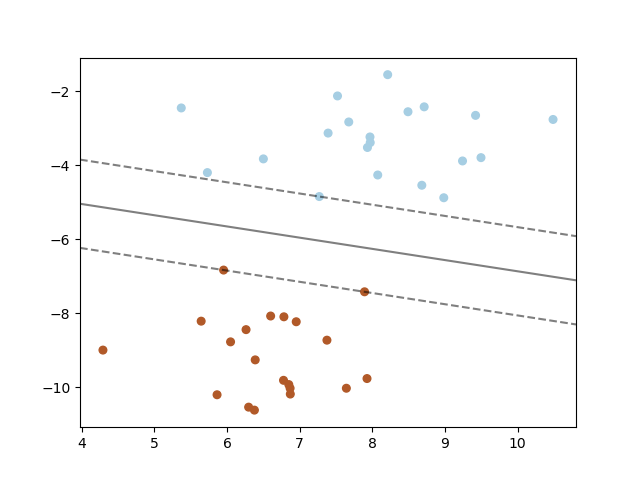
\includegraphics[width=0.5\textwidth]{images/svm_hiperplane}%
      \caption{Plano de separación de clases generado por una SVM}\label{fig:svm}
      \end{figure}

  \subsection{Perceptron Multicapa (MLP)}
      \begin{figure}
      \centering%
      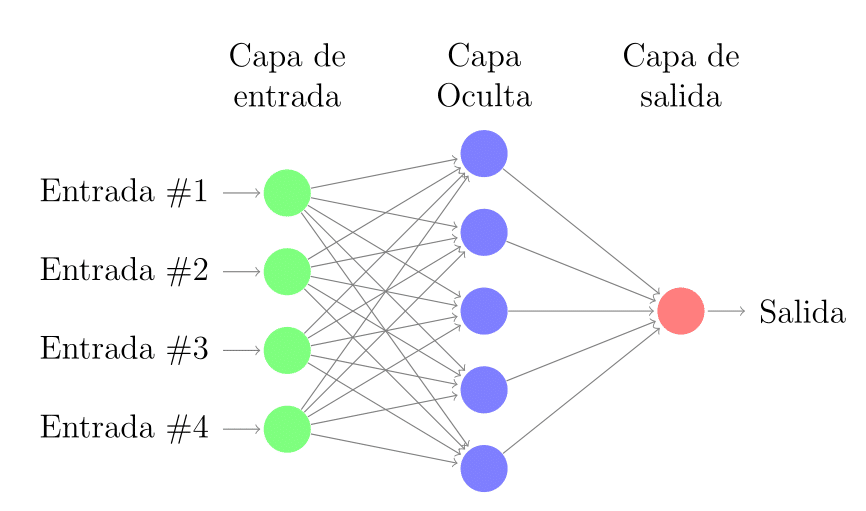
\includegraphics[width=0.7\textwidth]{images/ejemplo_mlp}%
      \caption{Arquitectura de una MLP de cuatro variables de entrada, una capa
              oculta de cinco neuronas y un sólo valor de salida}\label{fig:mlp}
      \end{figure}

    \par Un \textbf{Perceptron Multicapa} (MLP)\cite{mlp_intro1, mlp_intro2} es un tipo
      de red neuronal artificial (ANN) \textit{feedforward}.
      Éste es un algoritmo de aprendizaje supervisado que logra distinguir
      relaciones entre datos que no sean linealmente separables, aprende una función
      a partir de un conjunto de datos de entrenamiento y puede ser
      utilizada tanto para tareas de regresión como de clasificación haciendo uso, entre
      otras cosas, de una técnica llamada \textit{propagación hacia atrás}\cite{backpropagation}
      (\textit{backpropagation}, en inglés).
      El MLP consiste de al menos tres capas: una de entrada, una de salida y,
      como mínimo, una capa oculta\footnote{Una capa de neuronas artificiales que toman un conjunto
      de entradas ponderadas y producen una salida a través de una función de activación.};
      la vista gráfica de una arquitectura simple se puede observar en la
      Figura \ref{fig:mlp}.

    \par Una descripción matemática simplificada del algoritmo en cuestión es la
      que se menciona a continuación.
      Dados ejemplos de entrenamiento $(x_{1}, y_{1}), \dots, (x_{n}, y_{n})$
      donde $x_{i} \in \mathbb{R}^{n}$ y $y_{i} \in \{0,1\}$, un MLP de una capa oculta
      con una neurona aprende una función $f(x) = W_{2}g(W_{1}^{T} x + b_{1}) + b_{2}$
      donde $W_{1} \in \mathbb{R}^{m}$ y $W_{2}, b_{1}, b_{2} \in \mathbb{R}$ son
      parámetros del modelo. $W_{1}, W_{2}$ representan los pesos de la capa de entrada y la
      capa oculta, respectivamente. $b_{1}, b_{2}$ representan el sesgo agregado a
      la capa oculta y la capa de salida, respectivamente. La función
      $g(): \mathbb{R} \rightarrow \mathbb{R}$ es la función de activación, la cual
      es definida por defecto como la tangente hiperbólica. Está dada por,

      \begin{align}
        g(z) = \frac{e^{z} - e^{-z}}{e^{z} + e^{-z}}
      \end{align}

      En problemas de regresión, la salida del algoritmo es $f(x)$, por lo que la
      función de activación de salida es simplemente la función identidad. En estos
      problemas, MLP también utiliza como función de pérdida la correspondiente
      al \textit{Error Cuadrático}:
      \begin{align}
        Loss(\hat{y}, y, W) = \frac{1}{2} \norm{\hat{y} - y}^{2}_{2} + \frac{\alpha}{2} \norm{W}^{2}_{2}
      \end{align}

    \par Comenzando desde pesos con valores aleatorios, el MLP minimiza la función de
      pérdida actualizando repetidamente dichos pesos. Luego de calcular la pérdida,
      se propaga desde la capa de salida a todas las anteriores (\textit{backpropagation}),
      proporcionando un valor de peso a cada parámetros para disminuir la pérdida.
      Para ello, se utiliza \textit{descenso por gradiente}, en el cual el
      gradiente $\nabla Loss_{W}$ de la pérdida con respecto a los pesos es
      calculada y deducida de W.
      Más formalmente, es expresado como:
      \begin{align}
        W^{i + 1} = W^{i} - \epsilon \nabla Loss^{i}_{W}
      \end{align}
      donde $i$ es el paso de iteración, y $\epsilon > 0$ es la taza de aprendizaje.

      En general el algoritmo termina cuando se alcanza cierto número definido por el
      usuario de iteraciones o se cruza un humbral para la pérdida.

\end{document}
